\documentclass{article}
\usepackage{lipsum}
\usepackage[utf8]{inputenc}
\usepackage{braket}
\title{\underline {\textbf{Dimer solution of Hyperbolic Ising Model}}}
\author{Alapan Das}
\date{}%
\maketitle
%\usepackage{lipsum} 
\usepackage{biblatex} %Imports biblatex package
\addbibresource{bibtex.bib} %Import the bibliography file
\usepackage{appendix} % Package pour gérer les annexes
\usepackage{amsfonts}
\usepackage{xcolor}
\usepackage{amsmath}
\usepackage{graphicx}
\usepackage{physics}
\usepackage{hyperref}
\usepackage{url}

\hypersetup{
	colorlinks=true,
	linkcolor=blue,
	urlcolor=blue,
}

\begin{document}
	
	\textbf{Ising problem and Dimer Solution:} Our goal is to find the behavior of the spectrum of the Pfaffian matrix corresponding to the dimer model for the hyperbolic Ising model. In the presence of an external magnetic field, the usual dimer model mapping doesn't work as all the vertices can have any number of allowed edges. \\
	
	Having talked about the expansion, we see that our usual Fisher construction doesn't work as the points $x_i$ in $\langle{\sigma(x_1)\sigma(x_2)...\sigma(x_n)}\rangle$ has an odd number of edges but others have even. So we need to make the following modifications.\\
	
	
	\begin{center}
		\includegraphics[scale=1]{Dimer.jpg}\\
	\end{center}
	
	\vspace{0.5 cm}
	\pagebreak
	
	This is the diagram of the modified dimer configuration to find magnetization at some point $x\in G$ of the graph. That is $\mu_{\Lambda, \beta}=\langle {\sigma(x)} \rangle =\text{Pfaff}(\tilde{A})$, where $\tilde{A}$ is the Pfaffian matrix for modified graph. The modification just includes adding three points (blue) around the $x$-triangle and flipping the rule of dimer matching for just the center $x$-triangle. These three points act like mediators between the point $x$ and the others to make their opposite dimer matching rule consistent. So, for the edges of this region, weights are $v_{e}=1$. \\
	
	
	But this brings a global change to the Pfaffian orientation as we add an odd number of extra sites. As we have added three extra points, we may add one extra site at the boundary to keep the total number of points on the graph even.\\ 
	
	
	\begin{center}
		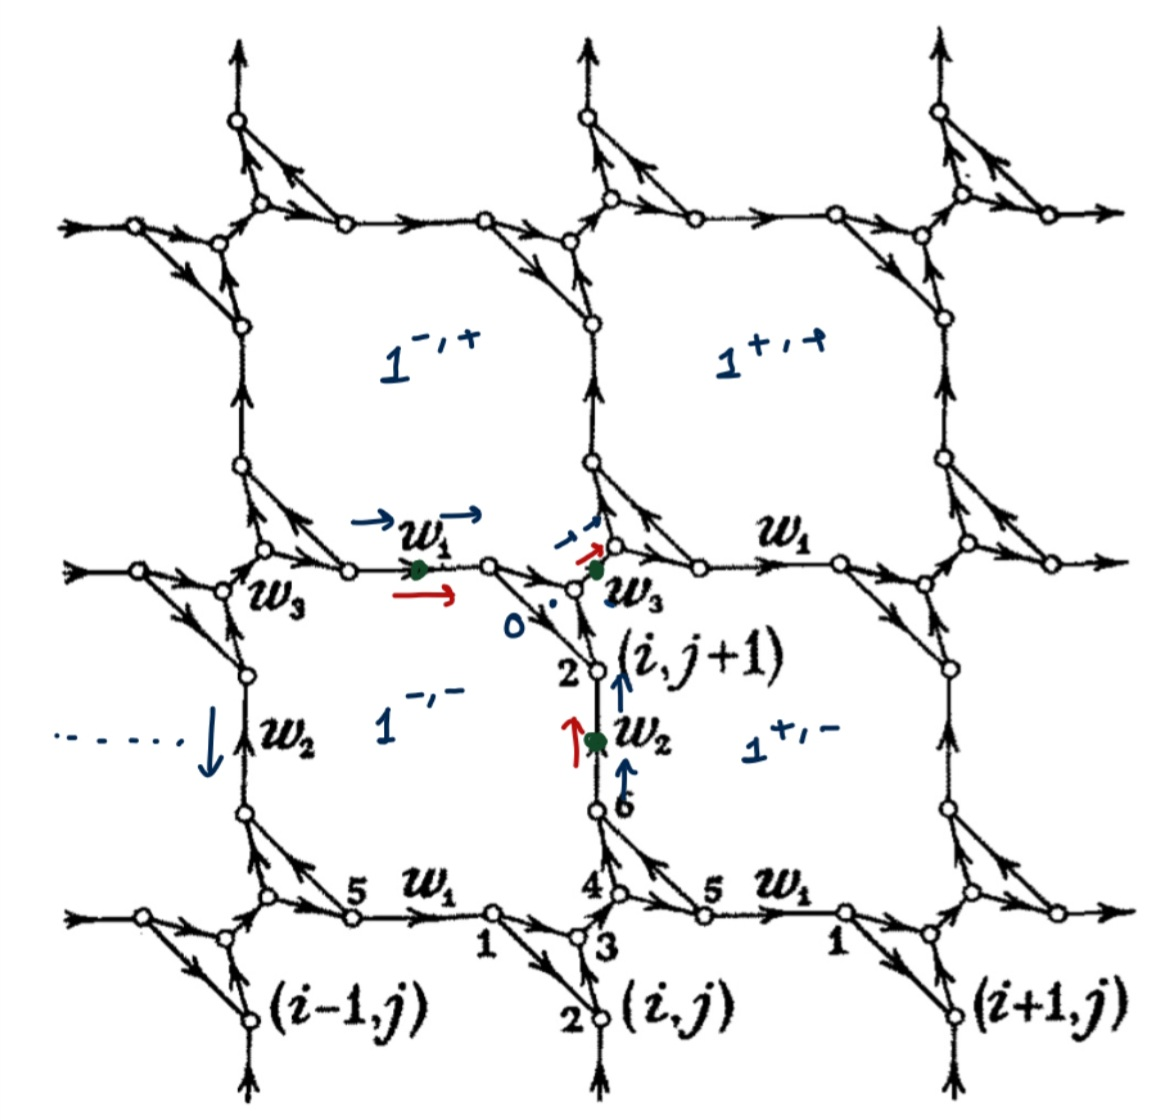
\includegraphics[scale=0.2]{pfaff mod.jpg}
	\end{center}\\
	
	
	
	This shows the orientation for the modified graph. The red lines (and the printed ones) are the original. The blue ones are after modification. So, there is a global orientation flip along a line as shown in the figure. This dimer configuration is not translationally invariant. We may join the extra legs at the corner or slightly modify the corners. We take two points for one corner and do not do any Fisher construction there. The dimer matching rule will be similar.\\ 
	
	We want to relate the spectrum of this matrix to the FK percolation as we can show that $=\mu^{+}_{\Lambda, T}=\langle{\sigma^{+}(x)}\rangle=\Phi^{w,p,2}[x \leftrightarrow \partial \Lambda ]$, where $\partial \Lambda$ is the boundary of the graph. This is equal to $\sum_{y \in \partial \Lambda} \langle{\sigma(x)\sigma(y)}\rangle$ for free boundary condition.\\
	
	Here, $\Phi^{w,p,q}(\omega)=\prod_{e\in \omega} p^{\omega(e)}(1-p)^{1-\omega(e)}q^{Cl(w)}$, here $Cl$ stands for number of connected components, $w(e)=0,1$ for closed or open edges and $w$ stands for wired boundary condition, that is all the boundary sites are connected. Here, $p \equiv 1-e^{-2\beta J}$.\\
	
	When $p=0$, there is no connected cluster; when $p=1$ there is only one connected cluster with probability 1. As the measure here is the number of connected clusters and not the total number of sites in those connected clusters, the FK measure $\Phi$ may not be monotonic in $p$. For amenable graphs, we can show that $\Phi[0 \leftrightarrow \partial \Lambda ] \leq e^{-c_pn}$ for $p<p_c$, similarly as Bernoulli percolation.  \\
	
	We want to understand the dependence of the spectrum of the Pfaffian of a modified Fisher graph for a hyperbolic lattice $(n,k)$. An important relation for any anti-symmetric matrix $A$ is $\partial_{\beta} \ln \text{Pf}(A)= \frac{1}{2}\Tr[A^{-1}\partial_{\beta}A]$. \\  
	
	\\	\vspace{0.2 cm}
	\textbf{Constructing the hyperbolic lattice and building its Pfaffian matrix:}\\
	\vspace{0.1 cm}
	
	The eigenspectrum is obtained by building the hyperbolic lattice with Pfaffian orientation. Below we write down in detail how we build the hyperbolic lattice. We have $|\lambda_{\text{max}}| \leq (\frac{1}{\tanh(\beta J)}+2)$.\\
	
	1) $(n,3)$ Hyperbolic lattice satisfies this recurrence relation: say $\alpha_g, \beta_g$ denotes the number of legged and legless nodes at the layer $g$. Then we can easily find the recurrence relation:$\alpha_{g+1}=(n-4)\alpha_g-\beta_{g} ; \beta_{g+1}=\beta_g$.\\
	
	2) For $n$ odd we give all the edges of the first layer clockwise orientations and for n even we set an odd number of them in that manner. All the radial edges/layer connecting edges are given radially outward orientations. At last rest of the edges are given appropriate orientations to satisfy the requirement of Pfaffian orientation. \\
	
	3) To build $g$-layer edges all the internal vertices of the original graph are expanded with triangles. Also, the layer connecting $\beta_{g}$ vertices of the last layer are expanded similarly. But other vertices of the last layer are expanded to only two edges as they have degree $2$. \\
	
	4) As the constructed Pfaffian is a real anti-symmetric matrix, all its eigenvalues are purely imaginary and come in complex conjugate pairs with $\text{Pf}(A)=\prod \lambda_{\geq 0}$. \\
	
	This is the link to the Python file for the written code: \href{https://github.com/ad1729-math/DP-Files/blob/main/Hyperbolic%20Pfaffian.py}{Hyperbolic Pfaffian}\\
	
	This file contains the code for the Pfaffian of a $(n,3)$ Hyperbolic lattice. Here we construct the lattice and its expander graph followed by the construction of the Pfaffian, the eigenspectrums of which we plot for various temperatures. \\
	
	\begin{center}
		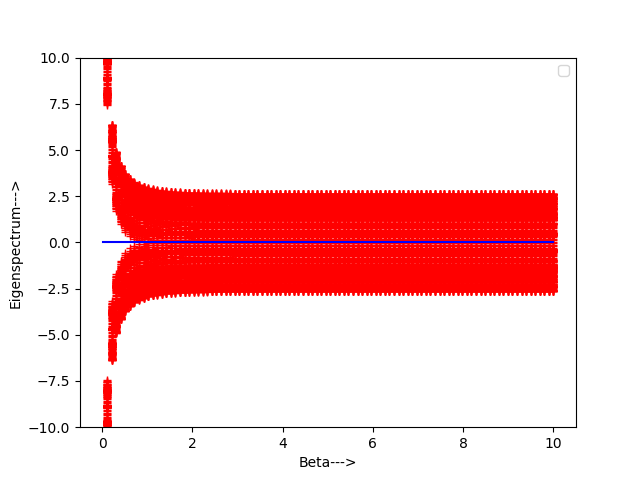
\includegraphics[scale=0.5]{Hyperbolic lattice eigenspectrum.png}\\
		\textbf{Figure-1:} For $K=\beta J \in [0.01,10]$\\
	\end{center}
	
	For finite $g$ surely the partition function is analytic and no eigenvalue should be zero. But in $g \to \infty$ limit the smallest absolute eigenvalue touches the zero line. Explicitly written we get, $Z(\beta, J)=2^{n(g)}(\sinh(\beta J))^{\xi(g)}\Delta(\beta, J)$.Where $\xi$ is the number of edges of the graph when there are $g$ layers. $\Delta$ is the Pfaffian generating function. $\Delta(\beta, J)=\sum_{m \in \mathcal{M}}\prod_{e \in m} v_e$. Here, $v_e=\tanh(\beta J)^{-1}$ for the original edges and $v=1$ for expanded edges.\\
	
	This can be seen that when $T \to \infty$, $Z \to 2^{\xi(g)}$ and for $T \to 0$, $Z \to (2^{n(g)}P(g))$ where $P(g)$ is number of perfect matchings for the expander graph.\\
	
	
	\begin{center}
		\includegraphics[scale=0.5]{Crossings 2.png}\\
		\textbf{Figure-3:} Observation of crossings ($g=4$)\\
	\end{center}
	
	\begin{center}
		\includegraphics[scale=0.2]{n=7 arm-chair boundary.png}\\
		\textbf{Figure-4:} n=7 spectrum for arm-chair boundary condition\\
	\end{center}
	
	\vspace{0.2 cm}
	\textbf{Comment:} There are two crossings at two different $\beta$. Those may indicate two-phase transitions.\\
	
	Below we plot $\ln (\text{Pf})(\beta, J)=\prod \lambda_{\geq 0}$ as function of $K=\beta J$ for $K \in [0.01,10]$. We see that the dimer partition function goes to the $T=0$ at around $K=2$. The green and red curves are for $2$ and $1$ layers respectively.\\
	\begin{center}
		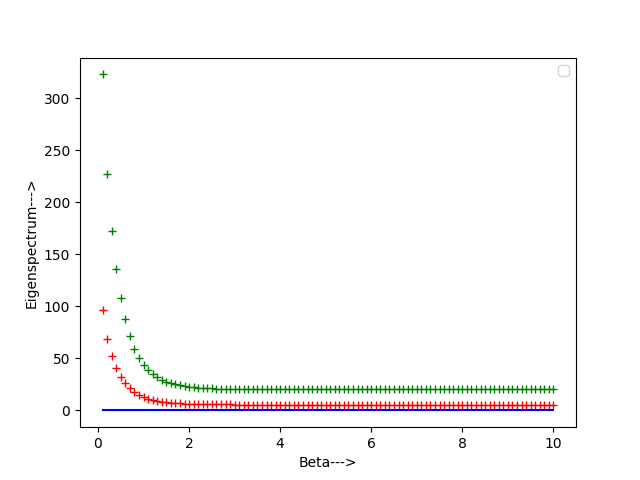
\includegraphics[scale=0.5]{Log Pfaffian.png}\\
		\textbf{Figure-5:} $\ln(\text{Pf})$ as a function of $K=\beta J$\\
	\end{center}
	
	
	\begin{center}
		\includegraphics[scale=0.3]{Hyperbolic Gens 4,3.png}\\
		\textbf{Figure-6:} Observation of crossings for $g=4$ (red) and $g=3$ (green).\\
	\end{center}
	
	We see that as we increase $g$ the lowest absolute eigenvalue goes closer and closer to zero even though the Pfaffian increases super exponentially with $g$ (as the number of perfect matchings increases exponentially with the number of edges and for hyperbolic graph, the number of edges is exponential in $f=g$). So, we see a phase transition. \\
	
	Now if we compare this to the 2-D Ising model which is an amenable graph we see that the eigenspectrum distribution in that case is like below:\\
	\begin{center}
		\includegraphics[scale=0.27]{2D Ising.png}\\
		\textbf{Figure-7:} $2$-D Ising model eigenspectrum\\
	\end{center}
	From the Fourier transform of the circulant anti-symmetric matrix, we get that the eigenvalues are: $\lambda(\theta, \phi, K)=\pm \frac{1}{v_1v_2v_3}\{1+(v_1v_2)^2+(v_2v_3)^2+(v_3v_1)^2-2[(1-v_1^2)v_2v_3\cos(\theta)+(1-v_2^2)v_3v_1\cos(\phi)+(1-v_3^2)v_1v_2\cos(2\pi-\theta-\phi)]\}$ where $v_1=\tanh(K_1), v_2=\tanh(K_2), v_3=\tanh(K^{*}), K=\beta J$. Here $K$ are for different types of bonds of the expander graph. At the end, we may take $v_1=v_2=\tanh(K)$ and $v_3=1$. From the expression of the eigenvalues we can see that at large $\beta$ limit the $(1-v^2)$ terms go to zero, hence all the eigenvalues merge to a single absolute value $\lambda_0=4$ which is exactly what we see in the graph. That is for the case of this amenable graph, there is a single zero touching point of the eigenspectrum, at $\beta J=\tanh^{-1}(\sqrt{2}-1)$ (the phase transition temperature).\\
	
	But this behavior is different in the case of the hyperbolic lattice. There we see that in any $\beta \geq \beta_0$ (the first touching point) the spectrum remains almost the same. Also, we observe a gap in the spectrum after the twist. \\
	
	\begin{center}
		\includegraphics[scale=0.2]{n=7 Spectrum 4 layers.png}\\
		\textbf{Figure-8:} Hyperbolic lattice eigenspectrum $g=4$ (Red) and $g=3$ (Green)\\
	\end{center}
	\vspace{0.2 cm}
	The plot for $n=6$ above was obtained for the orientation given in Fisher's paper. However, if we use our construction, we have the Pfaffian matrix a little different. As this is in Euclidean space, our construction is also translationally symmetric. So, doing Fourier transform we again plot the eigenvalues at different temperatures and obtain:
	
	\begin{center}
		\includegraphics[scale=0.27]{2D Ising Zoomed.png}\\
		\textbf{Figure-9:} Spectrum of $\mathbb{Z}_2$ lattice for our construction
	\end{center}
	
	Whereas if we calculate the full Pfaffian like we are doing in general for $5$ layers, then we get the following plot.\\
	
	\begin{center}
		\includegraphics[scale=0.27]{n=6 lattice.png}\\
		\textbf{Figure-10:} Spectrum of $\mathbb{Z}_2$ lattice\\
	\end{center}
	
	So, we expect the extra mesh-like points should go at $g \to \infty$ limit. Otherwise, the two graphs are similar. We observe a `twist' point here as well. The only thing different in the case of $n>6$ is the non-trivial sharp gap as shown in Figure-8.\\
	\vspace{0.5 cm}

	We get the plot for Figure-9 from the $6 \times 6$ matrices (Foruier transformed):  
	\begin{center}
		$A(r,s)=\begin{pmatrix}
			0 & -1 & 1 & 0 & -\omega_1 \phi_r^{-1} & 0\\
			1 &0&-1&0&0&\omega_2 \psi_s^{-1}\\
			-1&1&0&-\omega_3&0&0\\
			0&0&\omega_3&0&-1&1\\
			\omega_1 \phi_r&0&0&1&0&-1\\
			0&-\omega_2 \psi_s&0&-1&1&0\\
		\end{pmatrix}$\\
	\end{center}
	
	\vspace{0.2 cm}
	
	Here $\omega_i=v_i^{-1}$ and $\phi_r=\exp(\frac{2\pi r}{m}) , \psi=\exp(\frac{2 \pi s}{n})$. For square lattice $m=n$. The three bands on each side are due to this $6 \times 6$ matrices. The eigenvalues arriving with less density are expected to be due to the symmetry-breaking boundary condition that we have put in, i.e. we used two points expansion for the outer layer. \textbf{Triangular boundary condition has been checked}. We see that nice behavior for the analytic case because there we take Fourier transform ignoring the boundary effects, i.e. we assume $n \to \infty$ and remove the errors. In actuality we will be required four Pfaffians or else to continue with just one Pfaffian like this (planer) we will have to break the translational symmetry for the boundary sites (because to keep things planar, we require boundary connecting edges going around the whole lattice and connecting two sites sitting at opposite edges. Moreover, those edges will be enclosing other edges, so we lose symmetry). The analytical result that we discussed previously gives: $K_c=\beta_c J=\ln(\sqrt{2+\sqrt{3}})$ which also is found from the spectrum from the corresponding Pfaffian.\\
	
	Now we check different results when we scale the interaction strength as the metric of the hyperbolic space. As in the Poincare disc model, the distance of a point $z$ (in the unit disc) is $d(0,z)=2\tanh^{-1}(|z|)$. Approximating $d \approx g$ for $g$-th layer we write the interaction strength at $g$ layer as $J_g=\frac{J_0}{1-\tanh(g/2)^2}$. 
	
	\begin{center}
		\includegraphics[scale=0.2]{n=7 lattice 4 layers AdS metric.png}\\
		\textbf{Figure-11:} $(7,3)$ lattice for $4$ (Red) and $3$ (Green) layers with $\text{AdS}_2$ scaling\\
	\end{center}
	
	For other $(n,3)$ lattices we also see similar behavior and presence of such a gap. We may also want to check for self-dual lattices $(n,n)$ numerically or analytically (if possible, as in this case we get Kramer-Weiner duality).\\
	
	If we now remove the whole inner structure and only look at the last two layers we see the gap to be disappearing.\\
	
	
	\textbf{Finding Correlation using the modified construction:} Now we modify the dimer construction of the Hyperbolic lattice as we had discussed to obtain the correlation function. Here we find the correlation between two non-legless points $x,y$ at layer $g_c$, i.e. $\langle \sigma_x \sigma_y \rangle=2^{n(g)}\sinh(\beta J)^{\xi(g)}\tilde \Delta(\beta, J, x,y)$ where the dimer partition function $\tilde \Delta=\text{Pf}(\tilde A_{x,y})$. Here $\tilde A$ is the corresponding modified Pfaffian matrix. \\ 
	
	Plotting the correlation functions we see the phase transition for different $n$ as predicted by Peierl's argument. But we see some rather interesting behavior of the Pfaffian eigenspectrum near the phase transition point. Also for the negative curvature cases, i.e. $n \geq 7$ the non-trivial gap in the spectrum persists.
	
	\begin{center}
		\includegraphics[scale=0.4]{Correlation Spectrum n=7.png}\\
		\textbf{Figure-12:} Correlation for $n=7$ when $|x-y|=3$ at layer 2\\
		
		\includegraphics[scale=0.4]{Correlation n=6 structure.png}\\
		\textbf{Figure-13:} Correlation for $n=6$ inner structure\\
	\end{center}
	
	From Pielel's argument, we know that for $\mathbb{Z}_2$ lattice the correlation falls exponentially when $\beta \leq \beta_c$ and is greater than a constant for any $x,y$. Mathematically we write $\langle \sigma_x \sigma_y \rangle \leq \exp(-c d(x,y))$ for $\beta \leq \beta_c$ and $\langle \sigma_x \sigma_y \rangle \geq C(\beta)$ otherwise. Here, $d(.)$ may be considered as the Manhattan metric. This behavior reflects the properties of percolation in $\mathbb{Z}_d$ lattice. We observe similar behavior in our construction which we plot below for the hexagonal lattice for $x$ and $y$ being on the 2nd layer and distance $3$ and $5$ apart.\\
	\begin{center}
		
		\includegraphics[scale=0.4]{Correlation function n=6.png}\\
		\textbf{Figure-14:} Correlation function for $n=6$ for $d=3$ (Green) and $d=5$(Red)\\
		
		\includegraphics[scale=0.4]{n=7 Correlation (3,6).png}\\
		\textbf{Figure-15:} Correlation function for $n=7$ for $d=3$ (Red) and $d=6$ (Green)\\
		
	\end{center}
	
	\textbf{Boundary Connected Tree:} In the paper by ...., they studied the Phase transition of the correlation on a tree. As a related model, we consider here the tree with boundary sites being connected, so loops are appearing which spread well into the bulk of the lattice and so we expect to see behavior similar to other Hyperbolic lattices. Though the full analytic solution is hard, we can construct the Pfaffian recursively and then use perturbation theory. On the other hand, we may find the partition function, and correlations using recurrence, which we find numerically. These recurrences simplify the problem significantly both analytically and numerically. \\
	
	
	For a tree of degree $k$ with the boundary being connected, we define three quantities as mentioned above: $Z_n, \sigma_n, \gamma_n$ the partition function, top node (generation $0$) to side (generation $n$) node correlation and two sides (generation $n$ nodes of opposite sides) correlation. Then we get the following complicated recurrence: \\
	
	\begin{align}
		Z_{n+1} &= \sum_{\omega} (v\sigma_n)^{N(\omega)}(v^* \gamma_n)^{|\omega|-N(\omega)} {Z_n}^{g_n-|\omega|} \tag{1.1} \\
		\sigma_{n+1} &= \sum_{\omega_0;\omega}(v\sigma_n)(v^\gamma_n)^{\omega_0-1}\Gamma_n(\Omega-\omega_0) \tag{1.2} \\
		\gamma_{n+1} &= \sum_{\omega_0,\omega_1;\omega}(v\sigma_n)^2(v^\gamma_n)^{\omega_0+\omega_1-2}\Gamma_n(\Omega-\omega_0-\omega_1) \tag{1.3}
	\end{align}
	
	Here $\omega$ is a selection of different sets from the $k$ graphs of $n$-th layer. $\omega_{0,1}$ denote the number of $n$-layer graphs we select from left or right sides to recursively obtain the correlations in the next layer. $N(\omega)=2\text{# number of partitons in}\omega$. $g_n$ denotes the number of vertices of the $n$-layer graph. Lastly, $\Gamma$ implies all the loopings of the rest of the $n$-layer graphs that can be done similarly to what we do in the recursive process to get the partition function. \\ 
	
	For $k=2$ boundary-connected tree we have a much simpler form:
	\begin{align}
		Z_{n+1} &= Z_n^2+v^2v_1\gamma_n \tag{2.1} \\
		\sigma_{n+1} &= Z_n\sigma_n v^2+\sigma_n \gamma_n vv_1 \tag{2.2} \\
		\gamma_{n+1} &= \sigma_n^2v^2+\gamma_n^2 v_1 \tag{2.3} 
	\end{align} \\
	With the initial conditions being $Z_1=1+v^2v^*, \sigma_1=v+vv^* ,\gamma_1=v^*+v^2$.In all these cases $v=\tanh(\beta J), v^*=\tanh(\beta J_1)$.\\
	
	For this graph also we observe the non-trivial gap in the spectrum of the corresponding Pfaffian matrix of the expander graph. Similar to the above recurrence relation we build this Pfaffian matrix recurrently. \\
	
	If the matrix for $n$-th level is $A_n$ then the recurrence is as following: \\
	
	\begin{align}
		A_{n+1}=
		\begin{pmatrix}
			A_n & -B_n^T & C_n\\
			-B & O & \bar B_n\\
			-C^T & -\bar B_n^T &A_n
		\end{pmatrix}
	\end{align}
	
	\begin{center}
		\includegraphics[scale=0.5]{Boundary connected tree 9 layers.png}\\
		\textbf{Figure-16:} Gapped dimer spectrum for boundary-connected tree
	\end{center}
	
	This non-amenable graph has mirror symmetry along the axis that passes through the top node. But this graph is not fully symmetric which we see from the recurrence relation of the matrix. We may try to look analytically at how the spectrum depends on $n$ and why this gap due to bifurcation occurs. Naive perturbative calculation shows that the first-order correction is zero for all the eigenvalues. We call this naive as the order parameter $\omega>1$ which makes perturbation quite useless. So, to analytically learn about this we may look at the famous Sierpi\'nski triangle. \\
	
	$\textbf{Sierpi\'nski Triangle Graph:}$ The Sierpi\'nski triangle is one of the most famous fractal structures. For our purpose, we build the triangle from the ground up. Let all the edges have clock-weise orientations when looked from inside and the three legs coming out have radially outward orientation. So, $A_0$ is a $6 \times 6$ matrix corresponding to the expander triangle. Hence we have, 
	
	\begin{align}
		A_1=
		\begin{pmatrix}
			0&-\omega&0&0&0&0\\
			\omega&0&1&0&-1&0\\
			0&-1&0&\omega&1&0\\
			0&0&-\omega&0&0&0\\
			0&1&-1&0&0&\omega\\
			0&0&0&0&-\omega&0
		\end{pmatrix}
	\end{align}
	and 
	\begin{align}
		A_{n+1}=
		\begin{pmatrix}
			A_n&B_n&-B_n^T\\
			-B_n^T& A_n &B_n\\
			B_n & -B_n^T & A_n\\
		\end{pmatrix}
	\end{align}
	
	$A_{n+1}$ is a circulant block matrix, the eigenvalues of which are $\lambda_{n+1} = \{\text{eig}[ A_n+e^{\frac{2\pi i k}{3}}B-e^{-\frac{2 \pi i k}{3}}B^T]\}; k=0,1,2$. As the triangular blocks are connected only at their endpoints, the form of $B_n$ is:
	$\begin{pmatrix}
		0&0&\cdots&0&1\\
		0&\cdots&\cdots&0&0\\
		\vdots&\cdots&\cdots&\cdot&\vdots\\\
		0&0&\cdots&0&0\\
	\end{pmatrix}$. \\
	
	\textbf{This is to be investigated analytically.}
	
	\begin{center}
		\includegraphics[scale=0.5]{Sierpinski Graph Ising + half.png}\\
		\textbf{Figure-17:} Sierpinski spectrum for $5$-th generation \\
	\end{center}
	
	\textbf{Magnetization:} We discussed that the Dimer problem of the Ising model only works for zero magnetic fields. With a modification of the model that we had discussed we at most can find the correlation functions $\langle \sigma_{x_1}\sigma_{x_2}...\sigma_{x_{2r-1}}\sigma_{x_{2r}}\rangle$ at zero magnetic field. The magnetization however is defined as $\lim\limits_{h \to 0^{+}} \partial_h \ln[Z(\beta, h)]$. This $Z(\beta,h)$ can't be Taylor expanded for $\beta >\beta_c$. Hence we take a different approach to define magnetization. \\
	
	Let us fix a particular spin at $x \in \Lambda$. As $e^{KX}=\cosh(K)+\sinh(K)X$ for $X \in \{-1,1\}$. So, the breaking in curves works again. Because the spin at $x$ is now fixed to $+$, we do not get zero anymore when $\sigma_x$ has odd power, i.e. an odd number of curves pass through this. In this particular case, however, because there is no other such spin, all of them have to have an even number of curves passing, forcing $x$ also. So,  $Z[\beta | \sigma_x=1]=\frac{1}{2}Z(\beta)$. This also can be seen directly from symmetry. \\
	
	For multiple such fixed spins, say $\mathcal I= \{x_1,x_2,...,x_r\}$ all set to $+$ or $-$ spins. Diversity in signs of these sites will make things a little complicated as we will have to keep track of the signs. Then $Z[\beta | \mathcal I]=\frac{1}{2^{|\mathcal I|}}\sum_{\omega} \langle \prod_{y \in \omega} \sigma_y \rangle$. Here $\omega$ are set of all combinations of even number of those points, i.e. $\omega=\{\{\sigma_{x_{i_1}},\sigma_{x_{i_2}},...,\sigma_{x_{i_{2r-1}}},\sigma_{x_{i_{2r}}}\} | 2r<|\mathcal I|\}$.\\ 
	
	To define magnetization, we need to break the $\mathbb Z_2$ symmetry. One is what we just mentioned, find $Z(\beta,h)$ and let $h \to 0^{+}$. In another way, we may set the whole boundary or even just one site and find the corresponding magnetization, $\langle \sigma_0 \rangle$. For the latter case we will then have $m_0^{+,x}(T)=\mathbb{E_{\beta}}[\sigma_0 | \sigma_x=+]=\frac{1}{2}\langle \sigma_0 \sigma_x\rangle$. \\
	
	Duminil-Copin et.al. proved that at $|\Lambda| \to \infty$ limit, $m_0^{+}=\mathbb{E_{\beta}}[\sigma_0| \partial \Lambda=+]=m_0$. As we have seen, this can be expressed simply as the sum of combinations of correlation functions. (Have to look for non-amenable graphs).\\
	
	\textbf{Correlation scaling behavior:} For $\beta<\beta_c$ (specifically $K=0.1,0.3$) we find out plot the correlation function behavior as $\langle \sigma_x \sigma_y\rangle \sim e^{-\nu|x-y|}$. We find, for $n=6, \nu=1.94487786, n=7, \nu \approx 1.25165609$ and $\nu \approx 1.31234$ for $n=7$ anti-ferromagnetic case. \\
	
	
	$\textbf{Anti-ferromagnetic case:}$\\
	
	 In anti-ferromagnetic case $J<0$, which implies that the high temperature expansion is $Z=2^N\cosh(\beta |J|)^{|E|}(\sum_{\gamma_e} |v|^{|\gamma_e|}-\sum_{\gamma_o} |v|^{|\gamma_o|})$ , where $\gamma_{e,o}$ are loops of even or odd lengths and $v=\tanh(\beta J) \leq 0$. So, the partition function is the same for those graphs where no odd loops are possible, e.g. $(2n,3)$ graphs. However, there is huge difference in correlation function: $\langle \sigma_x \sigma_y \rangle_{F} \geq \langle \sigma_x \sigma_y \rangle_{AF}$. In the anti-ferromagnetic case, we see every behavior of the spectrum, i.e. the lowest eigenvalues touch zero at $\beta$ very large.\textbf{Is that infinite $\beta$? Need to check}.
	
	\begin{center}
		\includegraphics[scale=0.2]{n=7 anti-ferromagnetic.png}\\
		\textbf{Figure-18:} $n=7$ AIM spectrum
		\includegraphics[scale=0.5]{n=7 Correlation AIM.png}\\
		\textbf{Figure-18:} $n=7$ AIM correlation function
	
	\end{center}
	
	$\textbf{Describing the large $\beta$ boundary effect}$: \\

	
	
\end{document}
